\documentclass[10pt,a4paper]{report}

\usepackage[utf8]{inputenc}
\usepackage{amsmath}
\usepackage{amsfonts}
\usepackage{amssymb}
\usepackage{algorithm}
\usepackage{algpseudocode}
\usepackage{graphicx}
\usepackage[toc,page]{appendix}
\usepackage{float}
\usepackage[left=2cm,right=2cm,top=2cm,bottom=2cm]{geometry}

\author{Braydan Newman - n11272031}
\title{%
  Empirical Algorithm Analysis \\
   Efficiency of the in-order traversal algorithm  \\
  \large CAB301 - Assessment 2}
\date{}

\begin{document}
\maketitle
\tableofcontents
\pagebreak 

\section{Introduction}
In this empirical investigation, the primary aim is to assess the operational effectiveness of the in-order traversal method applied to a binary search tree (BST). The goal lies in determining the traversal process's efficiency class through counting the basic operations performed. The ratio of this count to the number of nodes in the Binary Tree determines the efficiency class. 

\section{Purpose of the Empirical Study}
The objective of this empirical analysis of algorithms is to formulate a hypothesis regarding the time complexity class of the in-order traversal algorithm presented in Appendix A. 

\section{Efficiency Metric to be Measured}
The efficiency metric used in this empirical algorithm analysis is the number of times the algorithm’s basic operations are performed. These basic operations include: 
\begin{itemize}
	\item Adding of the current node’s tool to the ordered list of tools 
	\item Visiting a node in the Binary Tree  
\end{itemize}

\section{Implementation for Experimentation}
The algorithm was implemented in C\# and a counter was inserted into the algorithm implementation and this was used to count the total number of times the basic operations occurred the In-order traversal  implementation. 

\section{Generation of a Sample of Inputs}
A test program was written in C\# that generates random test data for the binary tree, the generated data is 20 sets at 20 different intervals, with the length of the set ranging from 1000 to 20,000 at intervals of 1000. In total 400 different sets where tested each set ranging in length from 1000 to 20,000. The C\# program can be found in Appendix C. 

\section{Running the Algorithm Implementation on the Sample Inputs and Recording Results}
For each of the 20 intervals the 20 tests where averaged to get 20 results, one for each interval of length of the dataset. Each test the counter was used to count the number of basic operations and then after each test the count was recorded, the collated results of this are shown in the table below.  The raw experimental results have been submitted through Gradescope. 
\pagebreak 

\subsection{Experimental Results}
Test Data Table of Results

\begin{table}[H]
\centering
\begin{tabular}[1]{cc}
\hline
\textbf{Number of Tools} & \textbf{Number of Operations (Avg)} \\ \hline
1000 & 2000 \\ \hline
2000 & 4000 \\ \hline
3000 & 6000 \\ \hline
4000 & 8000 \\ \hline
5000 & 10000 \\ \hline
6000 & 12000 \\ \hline
7000 & 14000 \\ \hline
8000 & 16000 \\ \hline
9000 & 18000 \\ \hline
10000 & 20000 \\ \hline
11000 & 22000 \\ \hline
12000 & 24000 \\ \hline
13000 & 26000 \\ \hline
14000 & 28000 \\ \hline
15000 & 30000 \\ \hline
16000 & 32000 \\ \hline
17000 & 34000 \\ \hline
18000 & 36000 \\ \hline
19000 & 38000 \\ \hline
20000 & 40000 \\ \hline
\end{tabular}
  \caption{Basic opperation count results of 20 sets of 20 interval ranges of random data}
  \label{fig:basicOpperationCountResults}
\end{table}

\section{Analysis of the Experimental Results}
As shown by the results of the test data, the number of operations is double the number of nodes/tools in the collection. This is to be expected, as in this traversal of the binary tree every node is visited at least once and, in this implementation, it is only visited once. As well as traversal, each nodes “tool” is added to an array, this is also a basic operation and must happen once on every node, making the basic operations per node be a ratio of 2:1, operation count to node count. 

\begin{itemize}
	\item \textbf{Traversal Operation:} Every node in the BST must be visited at least once during the in-order traversal. 
	\item \textbf{Addition Operation:} Every tool in each node in the BST is added to the array. 
\end{itemize}

This can be calculated as the following, let the efficiency function \(t(n)\) represent the total number of basic operations for \(n\) nodes in the binary tree. \(t(n)=cg(n)\) where \(c\) is a constant and \(g(n)\) is a simple function. Calculating the values of \(t(2n)\) and \(t(n)\) then calculating the ratio with \( \frac {t(2n)}{t(n)} \) using the results in table.

\begin{equation}
\begin{split}
	n = 1000 \\
    t(2n) = t(2000) = 4000 \\
    t(n) = t(1000) = 2000 \\
    \frac{t(2n)}{t(n)} = \frac{4000}{2000} = 2 
\end{split}
\end{equation}

This gives a ratio of 2:1, meaning the efficiency function is linear as doubling the number of nodes doubles the number of basic operations performed in this in-order traversal. 

\subsection{Empirical Observation}

The behaviour above shows a linear correlation with the Complexity being \(O(2n)\) which is then simplified to the complexity class \(O(n)\), the constant 2 is omitted from Big-\(O\) notation as it doesnt add much complexity when input sizes are very large. 

\appendix
\chapter{}
\section{Pseudocode}
\subsection{ToArray}
\begin{algorithm}[H]
\caption{ToArray()}
\begin{algorithmic}[1]
	\State $tools \gets []$
	\State $index \gets 0$
	\If{$root \neq null$} 
		\State $inOrderTraversal(root, tools, index)$
	\EndIf
	\State \Return  $tools$
\end{algorithmic}
\end{algorithm}

\subsection{In-Order Traversal}
\begin{algorithm}[H]
\caption{inOrderTraversal(node, tools, index)}
\begin{algorithmic}[1]
	\If{$node.leftChild \neq null$} 
		\State $inOrderTraversal(node.leftChild, tools, index)$
	\EndIf
	\State $index \gets index + 1$
	\State $ tools[index] \gets node.tool $
	\If{$node.rightChild \neq null$} 
		\State $inOrderTraversal(node.rightChild, tools, index)$
	\EndIf
\end{algorithmic}
\end{algorithm}

\section{Code}
\subsection{ToArray}
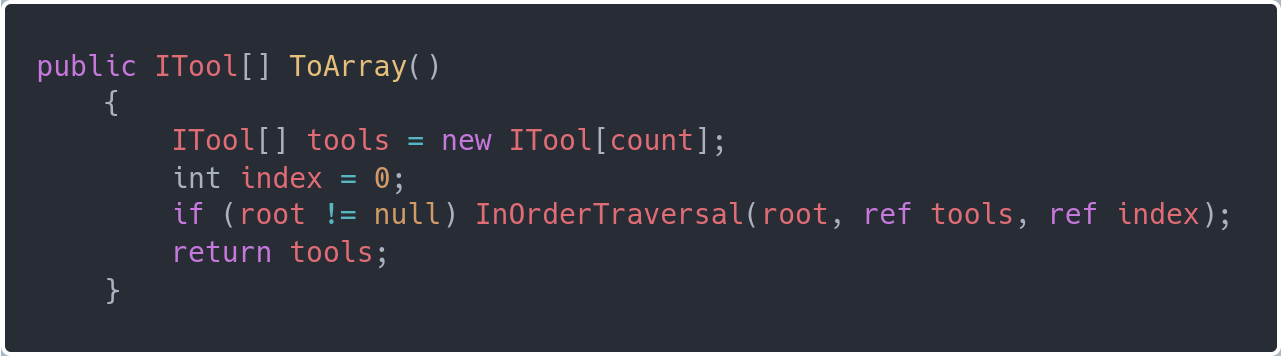
\includegraphics[width=\textwidth]{ToArray.png} 
\subsection{In-Order Traversal}
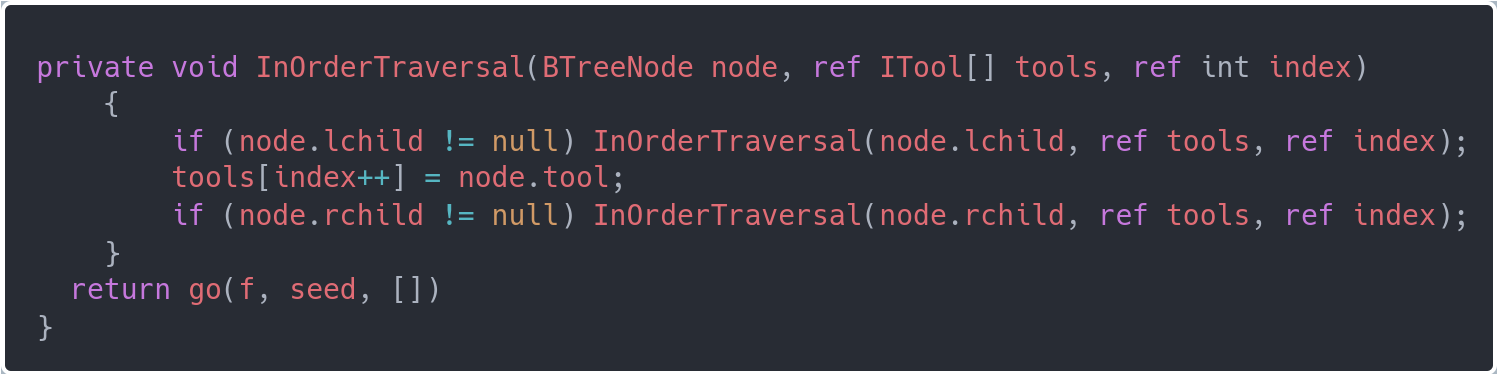
\includegraphics[width=\textwidth]{IOT.png} 
\subsection{Testing}
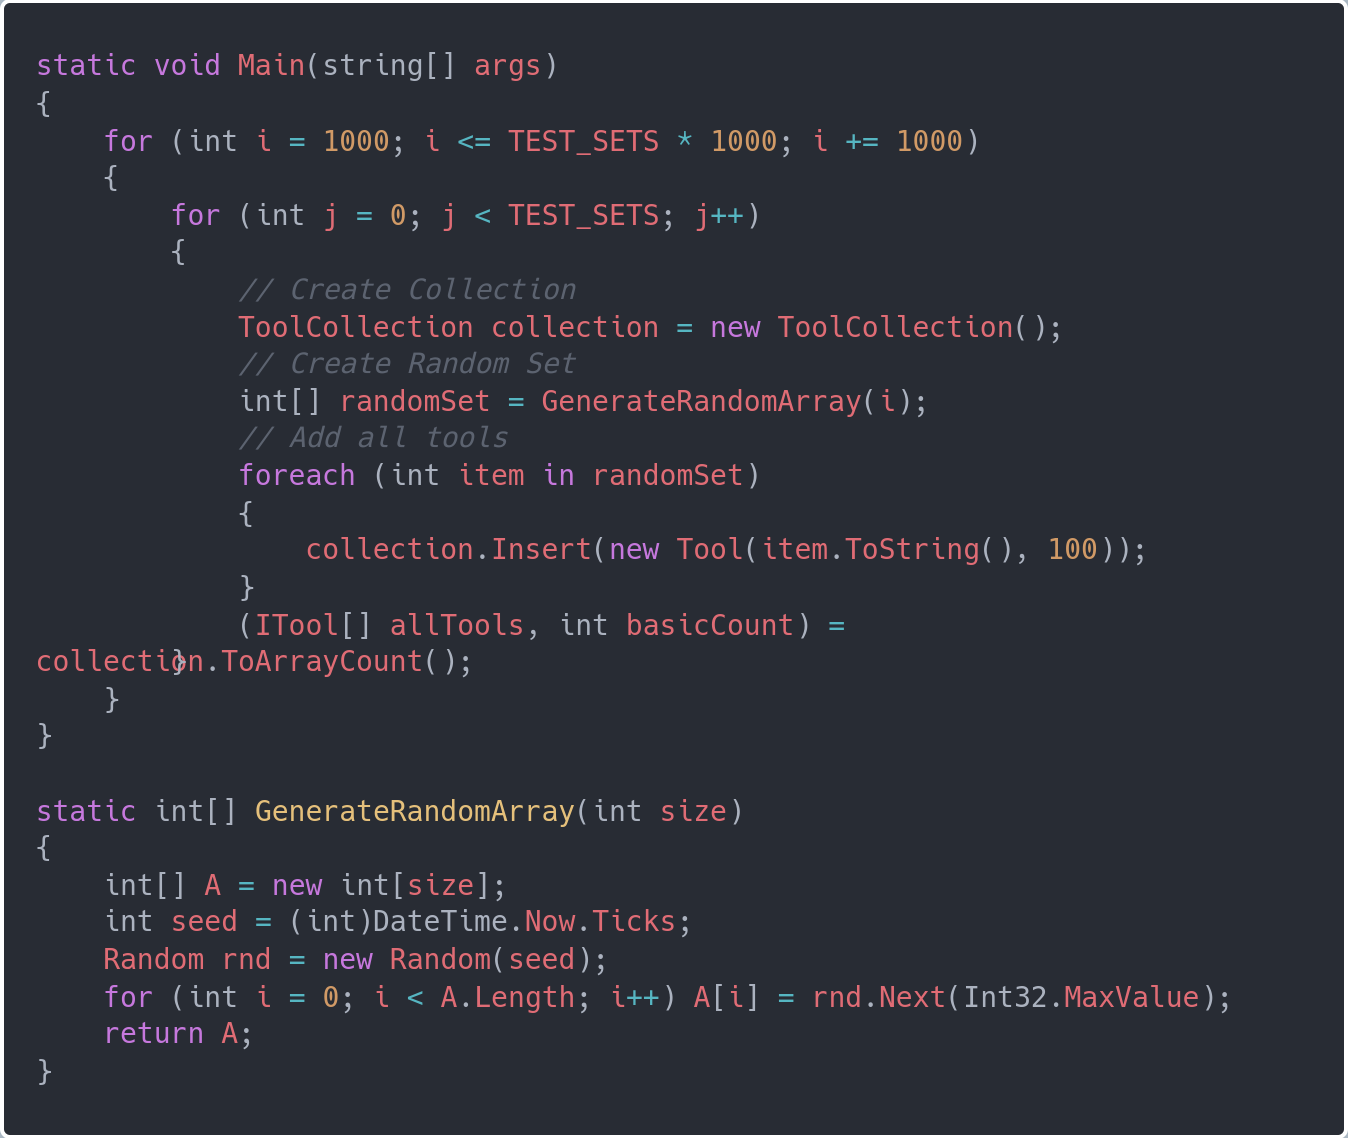
\includegraphics[width=\textwidth]{testing.png} 
\end{document}